%% -- mode: latex; mode: flyspell --
\documentclass[12pt, letter]{article}

%% Class name and Assignment number
%%
\newcommand{\courseName}{Scalable Matchmaking for Online Multiplayer Games}
\newcommand{\assignName}{CSC 562 - Distributed Systems Project}

%% Packages
\usepackage{amsmath,amsfonts,amssymb,amsthm,dsfont}
\usepackage{graphicx}
\usepackage[bookmarks=false]{hyperref}
\usepackage{color}
\usepackage{lipsum}
\usepackage{listings}
\usepackage{placeins}
\usepackage{geometry}
\usepackage{graphicx}
\usepackage{spverbatim}
\graphicspath{ {./images/} }
\geometry{
    letterpaper,
    %% total={216mm,279mm}, %< NSERC size
    margin=2.00cm,     %< default
    %% margin=1.87cm,       %< NSERC tightest
}

%% Headers and footers
\usepackage[explicit]{titlesec}
\newpagestyle{titlesec_assignment}{
  \sethead{\courseName}{}{\assignName}\setfoot{}{\thepage}{}
  \headrule
  %% \footrule
}

\begin{document}

%% Set header and footer
\pagestyle{titlesec_assignment}

%% Title
\title{\courseName\\\assignName}
\author{Sunil Kumar}
\maketitle

\section{Abstract}
The goal of this project is to make a good matchmaking system for online multiplayer games. Matchmaking in games can be defined as an art of matching a set of players together to maximize their enjoyment of the game. Google's Open source project Open-Match is already tackling this problem and is in alpha stage. So, the project is based on it to integrate a client and server with Open-Match to simulate a complete application including a game\_client, players, matchmaking system, server, etc. The final application will be deployed and running on a single Kubernetes cluster on Google Cloud Platform using the Kubernetes Engines in it. 

Final Project Demo Video:- https://youtu.be/d38UetVeEH0

\section{System Design}

System Architecture Diagram with arrows showing data flow (based on open match architecture):-

\centerline{
   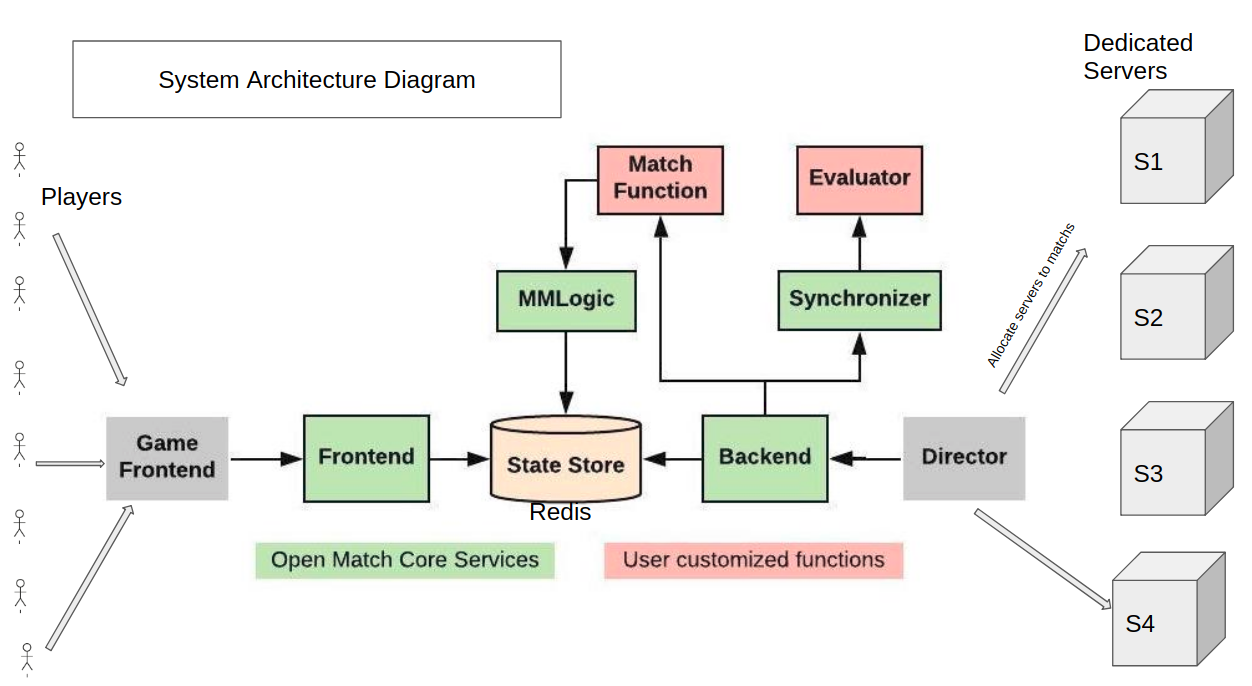
\includegraphics[width=0.8\textwidth]{images/arch2.png}
}

Below are the description of non-trivial components:-
\begin{itemize}
  \item Frontend: A service that handles tickets in open-match.
  \item Backend: A service that generates matches.
  \item Mmlogic: A gateway service that supports data querying in open-match.
  \item Match function: A service where your custom matchmaking logic lives in.
  \item Evaluator: evaluates proposed matches for there quality.
  \item Director:- back-end service which does communication between open match and dedicated game servers.

\end{itemize}

So, my dummy player's process, game client and director are part of the same service called om-demo written in Go language with a demo front-end using JavaScript and HTML to show whats going on in the system. The goal is to be able to have 1000 players playing concurrently without any issues. Lets now look at the technologies involved and deployment details in the next section.



\section{Implementation    and    Deployment}

Technologies used:-
\begin{itemize}
  \item \href{https://grpc.io/blog/coreos/}{gRPC with REST APIs}
  \item \href{https://swagger.io/}{Swagger UI} (Display framework for REST APIs)
  \item \href{https://golang.org/}{Golang}
  \item Docker
  \item Google Cloud Platform 
  \item Kubernetes (Google Cloud Kubernetes Cluster)
  \item \href{https://github.com/kubernetes/minikube/}{Minikube} (For creating local Kubernetes cluster on Virtualbox)
  \item \href{https://open-match.dev/site/}{Open-Match} (Google's open-source matchmaking framework for games)
  \item Make , Javascript, HTML etc.
\end{itemize}
\\
Following Technologies were part of open-match:-
\begin{itemize}
  \item Grafana (open source visualization tool)
  \item \href{https://prometheus.io/}{Prometheus} (open-source monitoring system)
  \item Redis
  \item \href{https://github.com/helm/helm}{Helm} (tool for managing Kubernetes charts)
\end{itemize}

\\

Flow Diagram of Demo using open match (source:- \href{https://open-match.dev/site/docs/getting-started/first_match/}{Open-Match Documentations}) :-
\\

\centerline{
   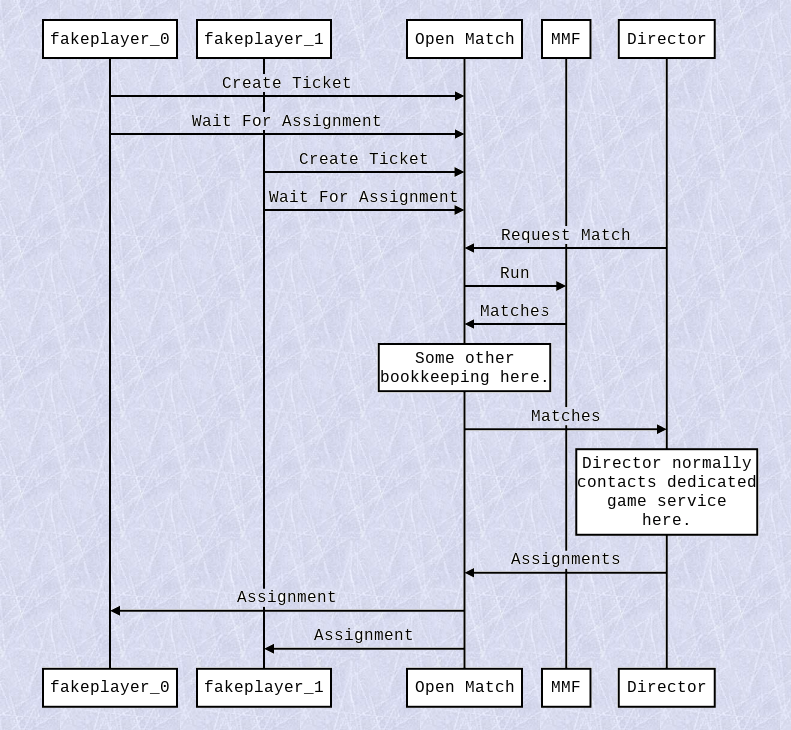
\includegraphics[width=0.6\textwidth]{images/DemoFlow.png}
}
\\

Legends in the above diagram:-
\begin{itemize}
  \item Assignment:- connection information to a game servers

  \item MMF:- Match Making Function i.e. service which selects players for a match after consideration for skill, latency, etc of the players in the pool (player currently looking for a match).
\end{itemize}

Let us see in the below diagram the high-level steps happen during matchmaking using open match (Source:\href{https://open-match.dev/site/docs/}{Open-match documentation}):-

\centerline{
   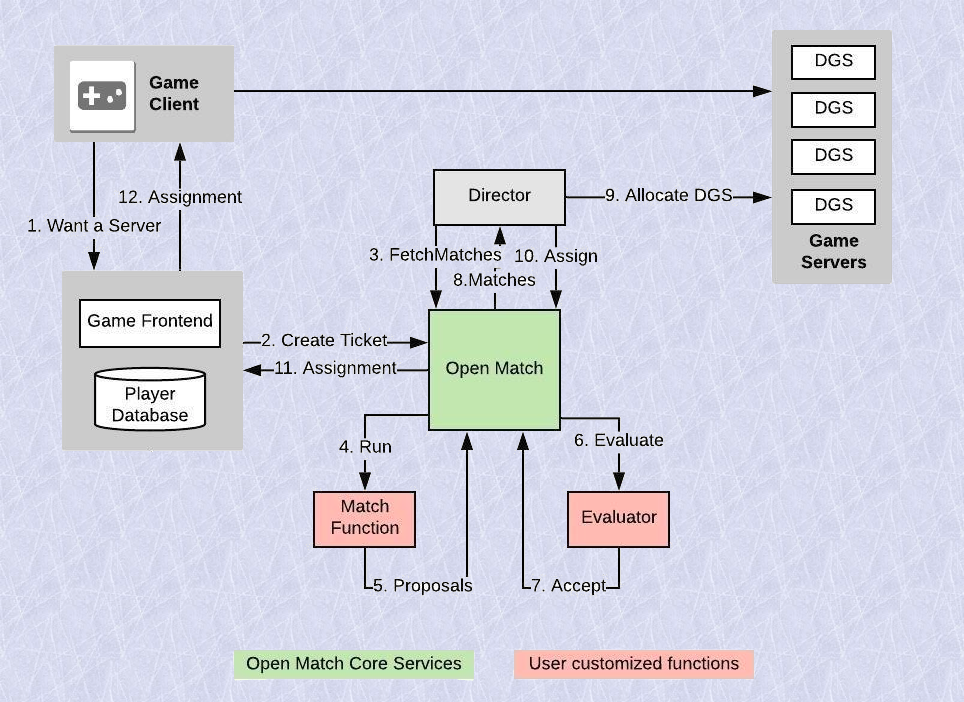
\includegraphics[width=0.6\textwidth]{images/DemoSteps.png}
}

We will be writing code to simulate the gray part in the above Diagram along with a custom Match Function which looks for 10 players for a match in Go language because client and server stubs are already generated for the gRPCs of Open-Match.

\\

For Deployment we move our docker images to google cloud Container Registry. Below screenshot shows the 2 images part of our demo in our Google Cloud Container Registry:-

\\
\centerline{
   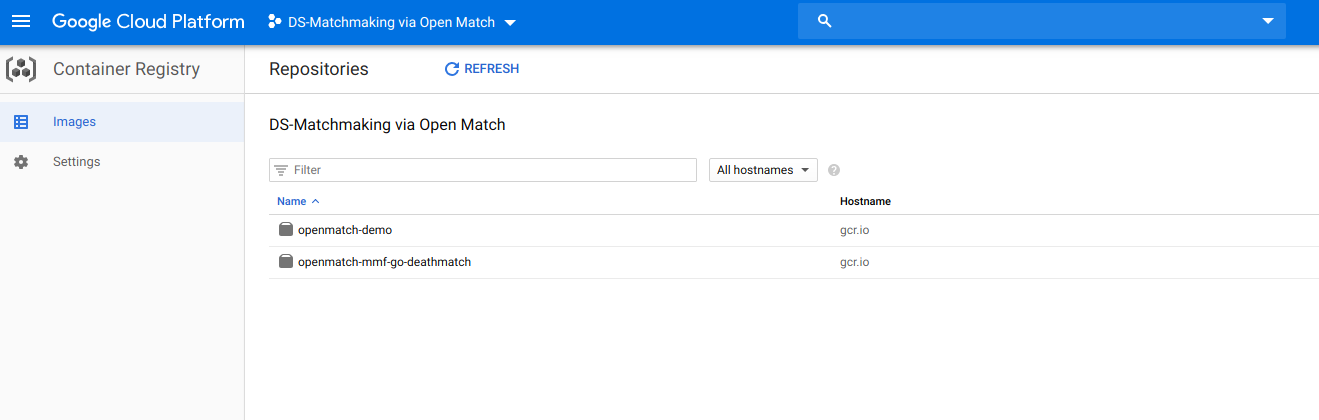
\includegraphics[width=1\textwidth]{images/uploadedImages.png}
}

Then we deployed our images in pods within the same cluster as other services of open-match. Below screenshot shows all services of open-match along with the demo and custom matchmaking service we deployed on the Kubernetes Cluster.

\centerline{
   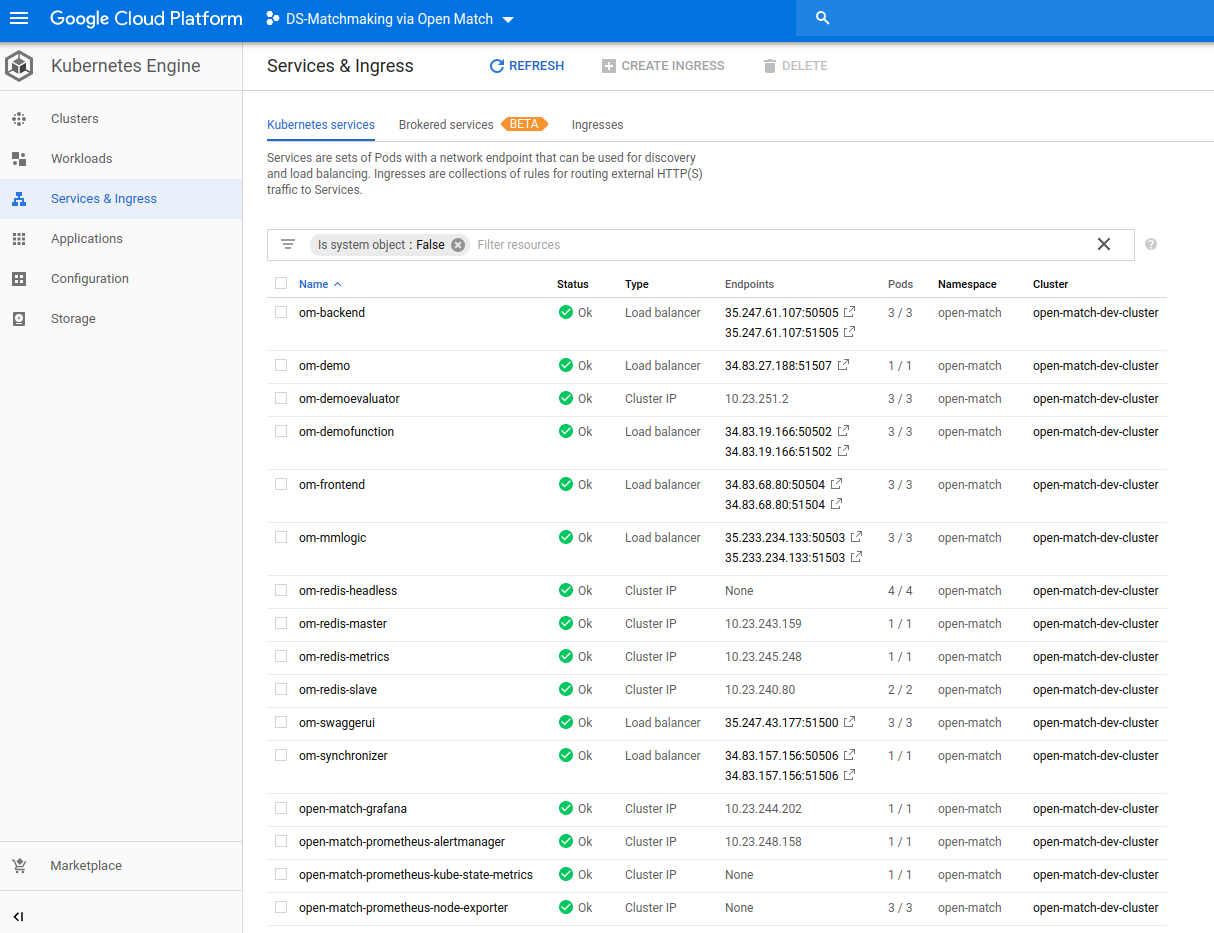
\includegraphics[width=.8\textwidth]{images/deploy.png}
}

Note some services which are not part of the core functionality of open-match had some errors (can be seen in demo video) and as Open-Match is in alpha stage some errors were expected. We started with 100 players and tried to scale up to 10000 players. More details of the evaluation in the next section.

\section{Evaluation}

To evaluate our matchmaking system we took 2 scenarios on the google cloud platform with 100 players and with 1000 players. It is important to note that because we have created our cluster using n1-standard-2 (2 vCPUs, 7.5 GB memory) at each node, our performance is limited by hardware also. when we tried setting up with 10,000 players on our demo, some of the services stop working and hence that scenarios were not compared. Below are the CPU load graphs of all 3 nodes in the cluster when running 100 and 1000 player respectively:-

\centerline{
   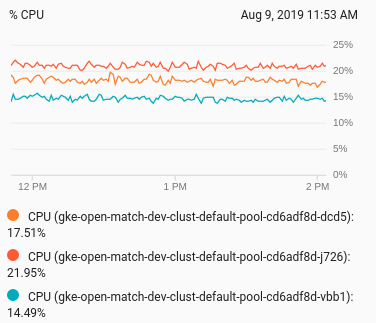
\includegraphics[width=.4\textwidth]{images/cpu100.png}
    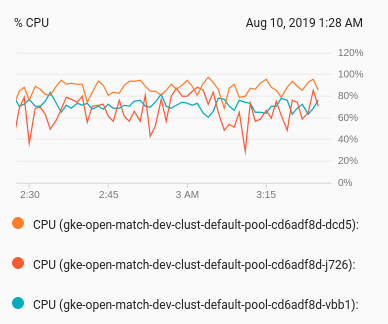
\includegraphics[width=.4\textwidth]{images/cpu1000.png}
}

From the above graph, it was clear that 1000 player playing on 100 servers is taking up to 95\% of the CPU usage and hence we cannot increase more on this hardware. Because we are using Kubernetes cluster which has Cluster Autoscaler feature this is not an issue. But due to lack of time and money, we did not explore this feature.

Now let us see the impact on network traffic when we move from 100 to 1000 concurrent players:-

\centerline{
   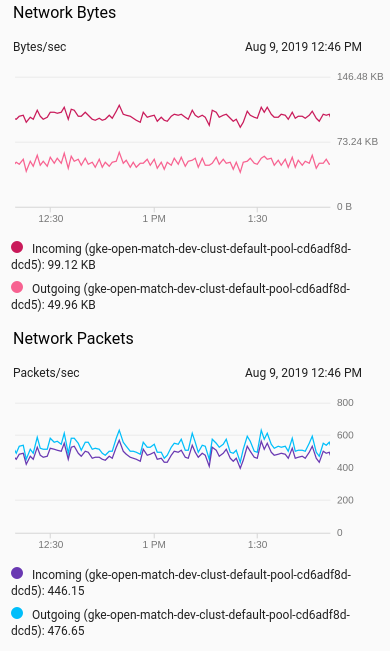
\includegraphics[width=.35\textwidth]{images/network100.png}
    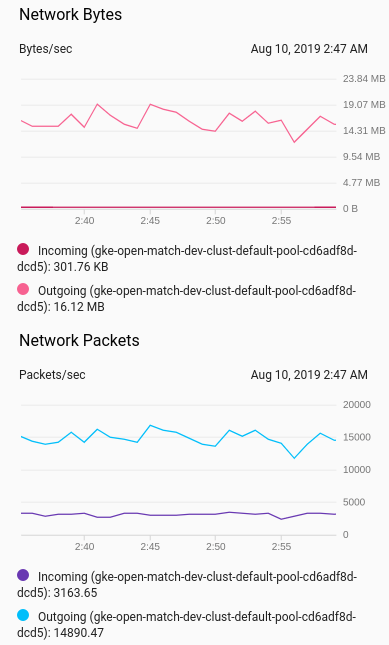
\includegraphics[width=.35\textwidth]{images/network1000.png}
}

\\
In the above graphs, we can see the increase in the network traffic when players count increase by 10 fold. Do note that the increase in network traffic is not strictly linear it seems because we note the number of packets was increase to 3200 packets per sec from 450 packets per sec whereas the outgoing traffic increased a lot up-to 15000 packets per sec from 500 packets per sec. We suspect that this might we due to our demo web-page fetching data to display. But the exact reason is not clear to us.

Note that the core services of open-match are deployed as load balancer mode with 1 process running at each node as shown in the below image. This ensures the Reliability of these services hence the whole system.

\centerline{
   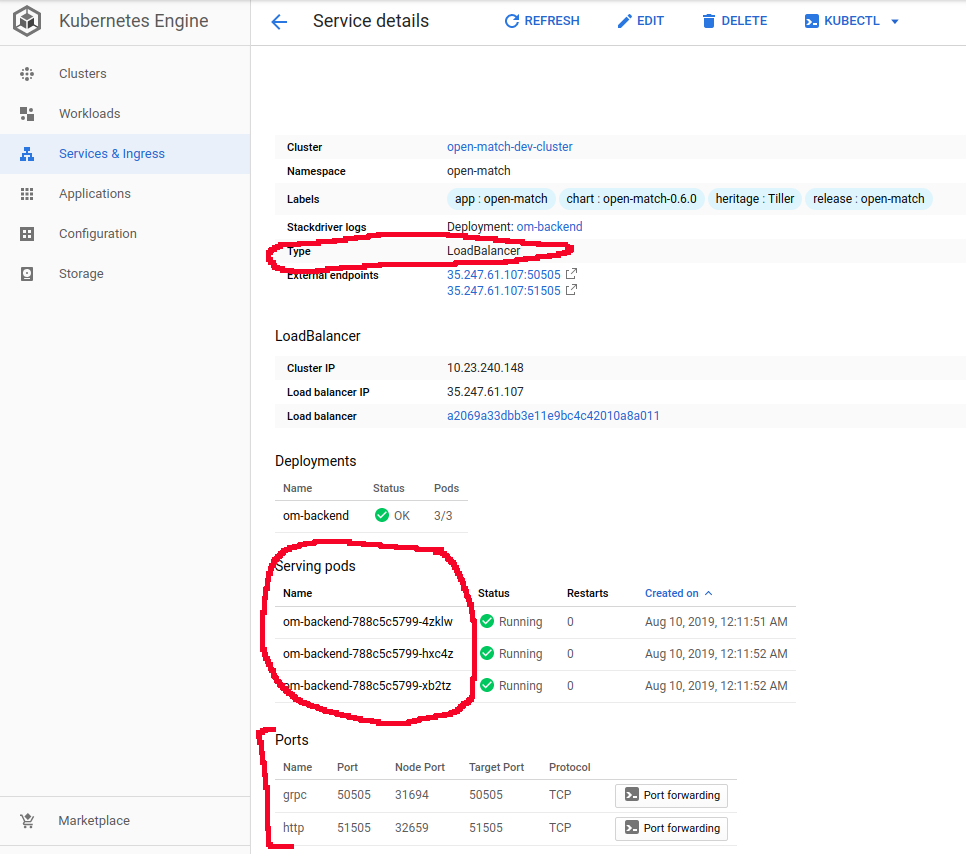
\includegraphics[width=.75\textwidth]{images/servicedetails.png}
}

We only had time to analyze our application APIs for one scenario using grafana with Prometheus monitoring service. Below graph shows the frequency of CreateTicket() API (either by REST or gRPC) is called on front-end service of open-match. Note this way we can analyze usage of any other API in our system. The image also shows the load is correctly balanced between the nodes for each API.

\centerline{
   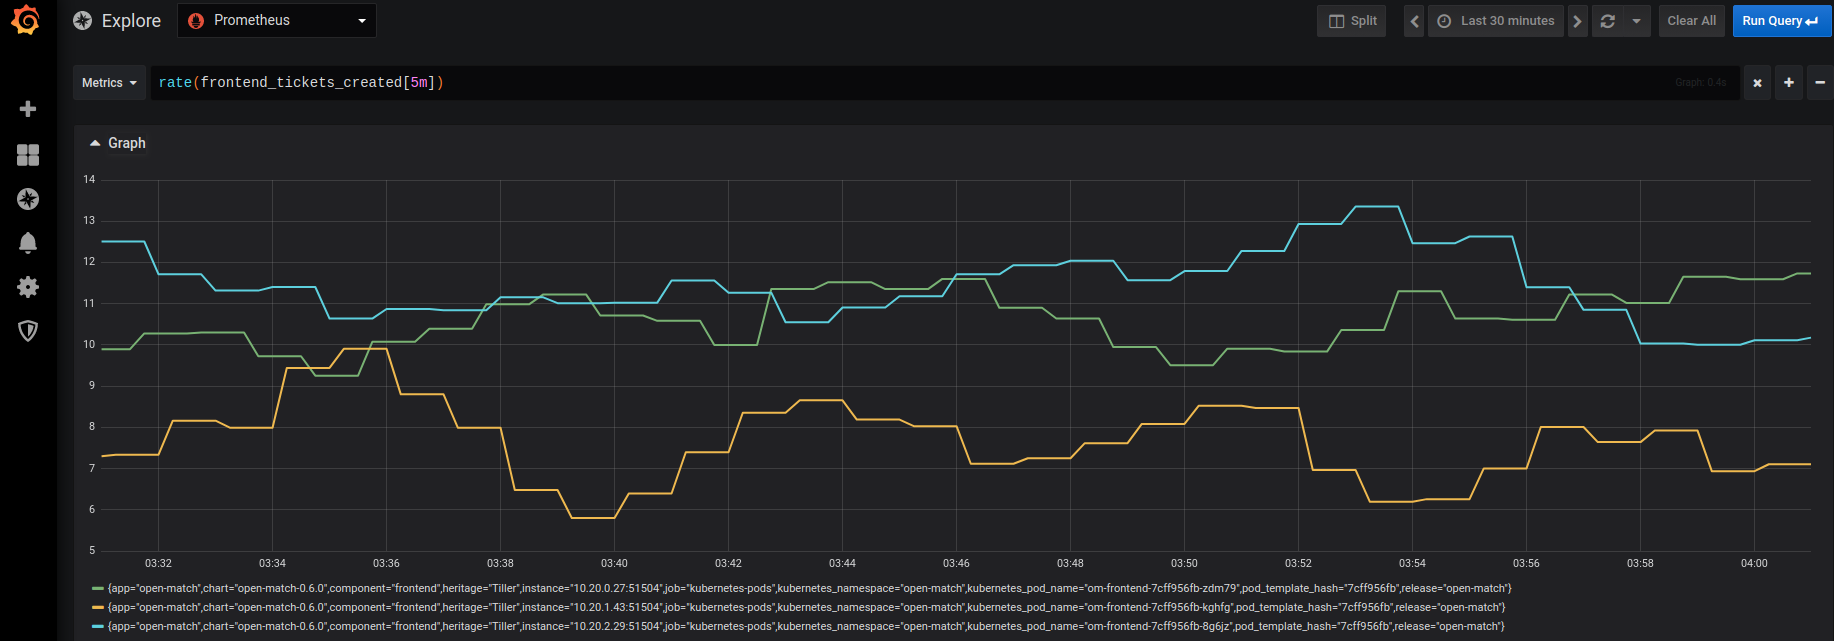
\includegraphics[width=0.75\textwidth]{images/frontendCreateT.png}
}

\\

Also while exploring grafana matrices we saw a lot of useful information can be fetched using it. For example CPU and memory usage by go processes, gRPC RTT, count, message size, etc. One of the interesting ones is shown below which shows the memory used by go processes which can be used to narrow down memory leaks or unwanted high member usage by any process:-

\centerline{
   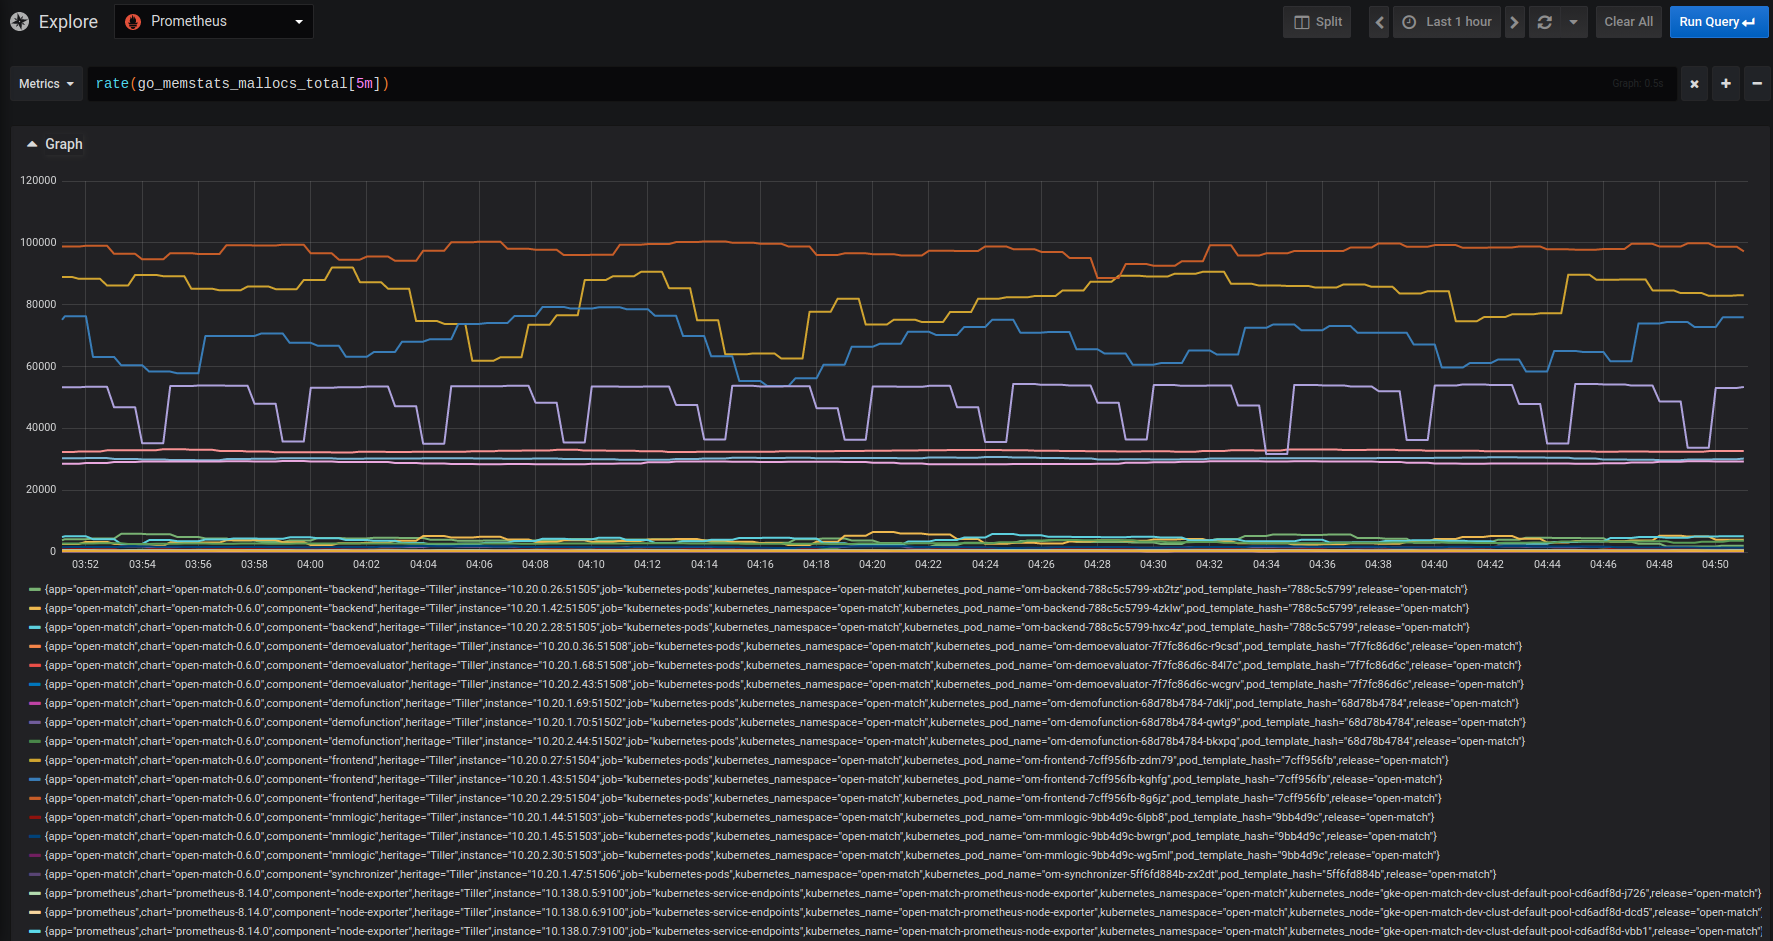
\includegraphics[width=0.75\textwidth]{images/gomemstats.png}
}

Open-match is designed as a micro-services pattern on kubernetes as the underlying platform which allow us to use kubernetes autoscaling feature to automate Scalability. It's highly Flexible because you can deploy it on any public cloud, local data center, or even on a local workstation. And it's also Extensible by adding custom matchmaking logic for any type of games. Kubernetes load balancer ensures reliability and high performance of the system.

\section{Discussion \& Future Work}

Good Performance of a matchmaking system is very subjective based on the game and type of mode you are playing. For example in-game like Dota and Fortnite where players are looking for competitive games matches, the system needs to focus on closely skilled players group together in a match. Whereas in other games the environment could be more casual and players only need new variety in matches focusing on social experience. The above evaluation is only done for vertical scaling i.e. higher number of concurrent players, a high number of requests, etc. There is also a need to fit-in complex game logic into the matchmaking functions. Open-match does support custom matchmaking function but analysis of such matchmaking system is very hard.

    While the open-match open source project moving toward a stable V1.0 build were all customizable components will fully support all languages etc. The future work of this project could be development and testing the performance of custom matchmaking function based on roles, MMR, etc. and compare the average wait time of the players. This could also include a custom evaluator to score the initial purposed matches and filter only good ones out of them.



\end{document}


%%% Local Variables:
%%% mode: latex
%%% TeX-master: t
%%% End:

